\documentclass{article}
\usepackage[a4paper,margin=2.5cm]{geometry}
\usepackage{amsmath}
\usepackage{tikz}
\usetikzlibrary{arrows.meta}
\begin{document}
\section*{Kesetaraan pecahan, desimal, dan persen dalam satu gambar}

Gambar berikut menunjukkan tiga wajah dari bilangan yang sama, $\tfrac{3}{4}$:

\begin{center}
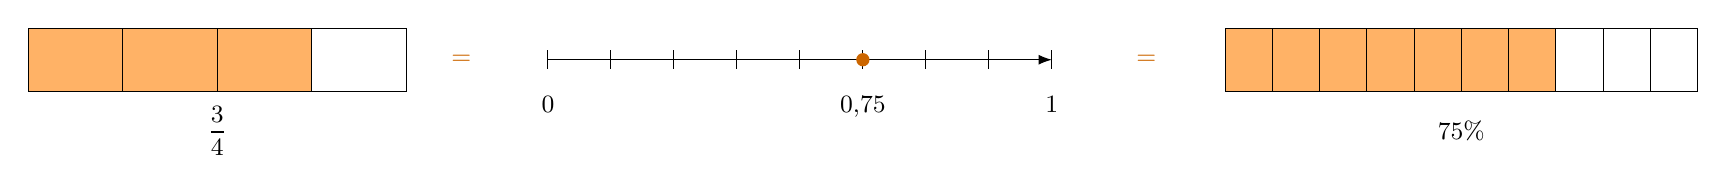
\begin{tikzpicture}[x=1cm,y=1cm,>=Latex,
  lab/.style={font=\small},
  acc/.style={text=orange!80!black,font=\small\bfseries}]
\begin{scope}[shift={(0,0)}]
  \foreach \i in {0,1,2,3}{
    \ifnum\i<3 \fill[orange!60] (\i*1.2,0) rectangle ++(1.2,0.8); \fi
    \draw (\i*1.2,0) rectangle ++(1.2,0.8);}
  \node[lab] at (2.4,-0.5) {$\dfrac{3}{4}$};
\end{scope}
\node[acc] at (5.5,0.4) {$=$};
\begin{scope}[shift={(6.6,0.4)}]
  \draw[->] (0,0) -- (6.4,0);
  \foreach \i in {0,...,8}{\draw (\i*0.8,0.12) -- (\i*0.8,-0.12);}
  \node[lab,below=7pt] at (0,-0.1) {$0$};
  \node[lab,below=7pt] at (4,-0.1) {$0{,}75$};
  \node[lab,below=7pt] at (6.4,-0.1) {$1$};
  \fill[orange!80!black] (4,0) circle (2.4pt);
\end{scope}
\node[acc] at (14.2,0.4) {$=$};
\begin{scope}[shift={(15.2,0)}]
  \foreach \i in {0,...,9}{
    \ifnum\i<7 \fill[orange!60] (\i*0.6,0) rectangle ++(0.6,0.8); \fi
    \draw (\i*0.6,0) rectangle ++(0.6,0.8);}
  \node[lab] at (3,-0.5) {$75\%$};
\end{scope}
\end{tikzpicture}
\end{center}

Kuncinya: ketiga representasi membagi sesuatu yang sama besar menjadi bagian
yang sama, lalu menghitung berapa bagian yang diambil. Batang pecahan membagi
satu kesatuan menjadi 4 bagian dan mengambil 3; garis bilangan menempatkan titik
pada 0,75 dari jarak 0 ke 1; pita persen membagi 100 kotak kecil dan mengambil 75.
Angka pembilangnya berbeda karena banyaknya potongan yang dipakai berbeda --
tetapi luas yang terarsir, letak titik pada garis, dan porsi pita itu persis sama.

\end{document}
